%%%%%%%% ICML 2026 SUBMISSION %%%%%%%%%%%%%%%%%
\documentclass{article}
\usepackage{microtype}
\usepackage{graphicx}
\usepackage{subcaption}
\usepackage{booktabs}
\usepackage{float}
\usepackage{hyperref}
\newcommand{\theHalgorithm}{\arabic{algorithm}}
\usepackage{icml2026}
\usepackage{amsmath}
\usepackage{amssymb}
\usepackage{mathtools}
\usepackage{amsthm}
\usepackage[capitalize,noabbrev]{cleveref}
\theoremstyle{plain}
\newtheorem{proposition}{Proposition}
\theoremstyle{remark}
\newtheorem{remark}{Remark}
\newcommand{\E}{\mathbb{E}}
\newcommand{\khat}{\hat k}
\newcommand{\pts}{\,\text{pts}}

\icmltitlerunning{The Winner's Curse of Automatic Prompt and Pipeline Search}

\begin{document}

\twocolumn[
  \icmltitle{The Winner's Curse of Automatic Prompt and Pipeline Search:\\
  What Post-Search Benchmark Scores Mean, and How to Report Them}
  \begin{icmlauthorlist}
    \icmlauthor{Anonymous Authors}{anon}
  \end{icmlauthorlist}
  \icmlaffiliation{anon}{Anonymous Institution}
  \icmlcorrespondingauthor{Anonymous}{anonymous@example.com}
  \icmlkeywords{prompt optimization, evaluation, selection bias, winner's curse, post-selection inference}
  \vskip 0.3in
]
\printAffiliationsAndNotice{}

\begin{abstract}
Automatic prompt and LLM-pipeline optimizers (DSPy-style compilers, best-arm-identification and minibatch searches) are routinely run on a benchmark's own questions, and the tuned system's score on those same questions is reported. We study what that number means. We prove that the optimism of the post-search score is at least the search regret and at most $\sqrt{\ln K/2n}$, and equals $\sigma_n\sqrt{1-\rho}\,m_K$ for equally good configurations with outcome correlation $\rho$. We then measure it on real LLM outcomes (Qwen2.5-0.5B/1.5B-Instruct and SmolLM2-1.7B-Instruct on MMLU-Pro; five search spaces of 40--80 prompt/format/demonstration configurations; five optimizer types; 2000 episodes per setting), where true accuracy is known by construction. With a 100-question dev set the reported accuracy exceeds the true accuracy of the selected configuration by 3.9--5.3 points (13--33\% of the accuracy) and exceeds even the best configuration's true accuracy in 74--90\% of episodes; the gap shrinks only like $n^{-0.6}$, grows with search effort much faster than the selected configuration improves, and is predicted within 10\% by a Gaussian plug-in. It distorts conclusions: a paired test declares a gain over an already-strong baseline in 14--19\% of episodes (nominal 5\%), reported lifts of 4.3--7.0 points over a mid-ranked baseline correspond to true lifts of 0.3--2.0 points, and a system searched over 32 configurations looks 3--10$\times$ better against one searched over 4 than it is. In a harness that tests eight reporting protocols against known truth, sample splitting is exactly unbiased but noisy and costs deployed accuracy; a search-replay bootstrap removes 70--80\% of the optimism for any optimizer; empirical-Bayes shrinkage is most accurate when configurations are exchangeable but fails with clustered quality levels; max-$t$ intervals are always valid but conservative. We give recommendations and discuss limitations (cached discrete search spaces, small models).
\end{abstract}

\section{Introduction}
\label{sec:intro}
Systems built from large language models are increasingly \emph{compiled} rather than hand-written: a developer states a task and a metric, and an optimizer searches over instructions, demonstrations, output formats or the structure of a multi-call program \citep{khattab2023dspy,opsahl2024optimizing,zhou2023large,yang2024large,shi2024efficient}. The search needs labelled questions, and in practice these are frequently the benchmark's own questions: the optimizer picks the configuration that scores best on a set of benchmark questions, and that best score on the same questions is then reported as the system's performance and used to compare systems. This is selection followed by evaluation on the data that drove the selection. Even when each configuration is only mildly better or worse than the others, the maximum over many noisy estimates is biased upward---the winner's curse \citep{smith2006optimizer}---so the reported number need not describe performance on new questions, and decisions based on it (``tuning gained $x$ points'', ``system A beats B'') can be wrong.

We ask two questions. \textbf{(Q1)} For a system whose configuration is searched on a finite set of questions and then used, how far is the reported score from its true accuracy on new questions, what controls the gap, and does it change conclusions drawn from reported scores? \textbf{(Q2)} Can reporting be made more reliable, and how should a reporting method be tested?

\textbf{Approach.} The gap is a property of the whole pipeline (data $\to$ search $\to$ report), so we study it by repeating the pipeline in worlds where the truth is known. We cache the correctness of 40--80 prompt configurations of real LLMs (Qwen2.5-0.5B/1.5B-Instruct, SmolLM2-1.7B-Instruct) on 450--750 real MMLU-Pro questions \citep{wang2024mmlupro}; taking the pool as the population gives exact true accuracies, and thousands of independent search episodes (five optimizer types imitating DSPy/MIPRO/best-arm-identification search logic) then measure the gap, its drivers, its effect on claims, and the bias/RMSE/coverage of eight reporting protocols. A short theory (\cref{sec:setting}) explains the results, and synthetic worlds isolate the factors.

\textbf{Findings.} (i) With $n{=}100$ dev questions the reported accuracy is $3.9$--$5.3$ points above the true accuracy of the deployed configuration---13--33\% of the accuracy itself---and above that of the \emph{best} configuration in the search space in 74--90\% of episodes, although the configurations differ by only 1--8 points (\cref{sec:exp}). (ii) The gap shrinks only as $\approx n^{-0.6}$, grows with the search effort (much faster than the selected configuration improves), with the number of effectively distinct configurations, and falls when one configuration is clearly best; a Gaussian plug-in predicts it within 10\%. (iii) It distorts conclusions: significance tests of a gain over a strong baseline fire 3--4$\times$ the nominal rate, mid-ranked baselines show lifts of $4.3$--$7.0$ points where the true lift is $0.3$--$2.0$, and systems tuned with unequal budgets are mis-ranked in magnitude. (iv) No protocol dominates: sample splitting is unbiased for any optimizer but noisy and costly; a search-replay bootstrap and empirical-Bayes shrinkage are far more accurate when their assumptions hold; a max-$t$ bound is always valid but wide.

\textbf{Contributions.} (1) A formal account of the post-search score with tight bounds and a plug-in predictor of its optimism (\cref{prop:opt,prop:cmp}). (2) A reusable meta-evaluation harness over cached real-LLM outcome matrices that measures bias, RMSE and coverage of reporting protocols with known truth. (3) A systematic measurement of this gap for LLM prompt/pipeline search on a real benchmark with real model outcomes, including its effect on lift and comparison claims. (4) A comparison of eight protocols and practical recommendations. Code, outcome matrices and all scripts are released.

\textbf{Conflict of interest disclosure.} None.

\section{Related Work}
\label{sec:related}
\textbf{Automatic prompt and program optimization.}
DSPy \citep{khattab2023dspy} compiles declarative LM programs by searching over instructions and demonstrations to maximise a user metric; MIPRO \citep{opsahl2024optimizing} does so for multi-stage programs with minibatch-based surrogate search; APE \citep{zhou2023large} and OPRO \citep{yang2024large} use an LLM to propose and refine instructions; \citet{shi2024efficient} cast prompt selection as best-arm identification under an evaluation budget. These works are concerned with how to \emph{find} a good configuration. We study what the score of the configuration found \emph{means} when the questions that guided the search are also used to score it, for a family of optimizers that includes simplified versions of each of these search strategies.

\textbf{Prompt sensitivity and LLM evaluation statistics.}
\citet{sclar2024quantifying} document large accuracy swings under meaning-preserving formatting changes, and \citet{polo2024efficient} estimate the distribution of performance over many templates from few evaluations; \citet{miller2024adding} argue for error bars that treat benchmark questions as a sample from a super-population. Sensitivity makes search worthwhile, and it also makes the selection effect we measure possible; error bars computed for a \emph{fixed} configuration do not account for it.

\textbf{Selection bias and adaptive data analysis.}
That the best of many noisy estimates is optimistic is the winner's/optimizer's curse \citep{smith2006optimizer}; in machine learning it appears as selection bias in model selection \citep{cawley2010overfitting,varma2006bias}, with bootstrap and CV-based corrections \citep{efron1997improvements,tibshirani2009bias} and a careful account of what cross-validation does and does not estimate \citep{bates2023cross}. When one dataset is queried adaptively, validity degrades with the number of queries; the reusable holdout \citep{dwork2015preserving,dwork2015reusable} and the Ladder \citep{blum2015ladder} limit the information released about the holdout, and \citet{recht2019imagenet} measured the accumulated effect of reuse by re-collecting test sets.

\textbf{Post-selection inference.}
Simultaneous intervals \citep{berk2013valid,chernozhukov2013gaussian}, conditional (truncated-Gaussian) inference \citep{lee2016exact}, and inference on the winner among many estimates \citep{andrews2024inference} give intervals for selected targets. We instantiate these ideas for prompt/pipeline search with outcome matrices from real LLMs and compare them with sample splitting, bootstrap, and empirical-Bayes corrections in a harness where the ground truth is known by construction.

\section{Setting: what a post-search score estimates}
\label{sec:setting}
\textbf{Setup.} A \emph{configuration} $k\in\{1,\dots,K\}$ is a complete prompt or LLM-program specification (instruction, demonstrations, output format, \dots). For a question $x$ from a benchmark distribution $P$, $Y_k(x)\in\{0,1\}$ is the correctness of the system under $k$ (with deterministic decoding; stochastic decoding only adds noise); $\theta_k=\E_P Y_k$ is its \emph{true accuracy}. A developer holds $n$ labelled questions $D$ drawn i.i.d.\ from $P$ and runs a search procedure $\mathcal A$ that queries outcomes $Y_k(x)$, $x\in D$, and returns a configuration $\khat$. The common practice we examine is to report the \emph{naive score} $\hat S=\frac1n\sum_{x\in D}Y_{\khat}(x)$. The target of interest is $\theta_{\khat}$, the accuracy of the deployed configuration on fresh questions; the \emph{gap} is $\hat S-\theta_{\khat}$ and the \emph{optimism} is $\mathcal O=\E[\hat S-\theta_{\khat}]$.

\textbf{Exhaustive search.} Let $\bar Y_k$ be the dev accuracy of $k$, $\epsilon_k=\bar Y_k-\theta_k$, $\khat=\arg\max_k\bar Y_k$, $\theta^\star=\max_k\theta_k$.
\begin{proposition}[Size of the optimism]\label{prop:opt}
(a) $\mathcal O\;\ge\;\theta^\star-\E[\theta_{\khat}]\;\ge 0$: the optimism is at least the expected regret of the search. (b) $\mathcal O\le \E\max_k\epsilon_k\le\sqrt{\ln K/(2n)}$. (c) If all $\theta_k$ are equal and $(\epsilon_k)$ is Gaussian with common variance $\sigma_n^2=\bar p(1-\bar p)/n$ and equal pairwise correlation $\rho$ (the correlation of per-question outcomes between configurations), then $\mathcal O=\sigma_n\sqrt{1-\rho}\;m_K$, with $m_K=\E\max_{k\le K}Z_k\le\sqrt{2\ln K}$ the expected maximum of $K$ i.i.d.\ standard normals ($m_{2}{=}0.56$, $m_{10}{=}1.54$, $m_{40}{=}2.16$, $m_{80}{=}2.43$).
\end{proposition}
\emph{Proof.} (a) $\E\hat S=\E\max_k\bar Y_k\ge\max_k\E\bar Y_k=\theta^\star$. (b) $\hat S-\theta_{\khat}=\epsilon_{\khat}\le\max_k\epsilon_k$; each $\epsilon_k$ is sub-Gaussian with variance proxy $1/(4n)$ (Hoeffding), so the maximal inequality gives $\sqrt{2\cdot\frac1{4n}\ln K}$. (c) Write $\epsilon_k=\sigma_n(\sqrt\rho Z_0+\sqrt{1-\rho}Z_k)$; the common part has mean zero and $\hat S - \theta = \max_k \epsilon_k$ since all $\theta_k$ coincide. $\square$

The optimism therefore (i) shrinks only as $n^{-1/2}$, (ii) grows with the number of configurations \emph{effectively} compared, $\sqrt{(1-\rho)}\,m_K$, so that highly correlated search spaces (as are small variations of one prompt) are less inflated than diverse ones, and (iii) is largest in units of $\sigma_n$ when configurations are equally good and decays as the true spread $\mathrm{sd}(\theta_k)$ grows relative to $\sigma_n$ (a ``signal-to-noise'' ratio $\mathrm{SNR}=\mathrm{sd}(\theta_k)/\sigma_n$): when one configuration is clearly best, selection is stable and there is little to be optimistic about. We check (c) and the SNR dependence in \cref{sec:exp}. For adaptive optimizers the same logic applies with the information the search extracts from $D$, which is more limited for budget-constrained searches (successive halving, minibatch search) than for exhaustive evaluation.

\begin{proposition}[Budget-confounded comparisons]\label{prop:cmp}
Let systems A and B be tuned on the same $D$ over disjoint spaces with $K_A>K_B$ equally good, equally correlated configurations. Then $\E[\hat S_A-\hat S_B]-(\E\theta_{\khat_A}-\E\theta_{\khat_B})=\sigma_n\sqrt{1-\rho}\,(m_{K_A}-m_{K_B})>0$.
\end{proposition}
\noindent The reported advantage of the system that was tuned harder is inflated even if tuning is equally effective for both; \cref{sec:exp} measures this on real outcomes.

\section{Reporting protocols and how we test them}
\label{sec:protocols}
Given an episode (labelled set $D$ of size $n$, optimizer, selected $\khat$), a \emph{reporting protocol} outputs a point estimate and, where defined, an interval for $\theta_{\khat}$. We compare eight protocols; all but sample splitting report on the \emph{same} deployed $\khat$ chosen with all $n$ questions.

\textbf{(P1) Naive.} $\hat S$ with a Wilson 95\% interval, i.e.\ the interval one would compute for a fixed configuration.
\textbf{(P2) Sample splitting.} Run $\mathcal A$ on $n_s=fn$ questions, deploy its choice $\khat_s$ and report its accuracy on the other $n-n_s$ questions (Wilson interval). It is exactly unbiased for $\theta_{\khat_s}$ for \emph{any} optimizer, but $\khat_s$ is chosen with less data.
\textbf{(P3) Cross-fitting.} $5$-fold: run $\mathcal A$ on four folds, score its choice on the fifth, average. This estimates the accuracy of the \emph{procedure} at $0.8n$ questions rather than that of the specific $\khat$ \citep{bates2023cross}; we measure against $\theta_{\khat}$.
\textbf{(P4) Search-replay bootstrap.} Rerun $\mathcal A$ on $B{=}100$ bootstrap resamples of $D$, estimate the optimism as the mean of (apparent accuracy on the resample $-$ accuracy on $D$) of the selected configuration, and subtract it (Efron-style); also the $.632$ variant that mixes in out-of-bag accuracy \citep{efron1997improvements}. It is optimizer-agnostic but requires rerunning the search (here free, as outcomes are cached).
\textbf{(P5) Empirical Bayes shrinkage.} Treat the true accuracies of the $m$ fully evaluated configurations as exchangeable draws from a normal prior; estimate its variance by moments from the dev means using the \emph{paired} sampling covariance of the configurations, and report the posterior mean of the winner. For an interval we use the posterior mean $\pm1.96\sqrt{u+v_{\hat k}}$, where $v_{\hat k}$ is the (unshrunk) paired sampling variance of the winner and $u$ the sampling variance of the grand mean (details in \cref{app:impl}).
\textbf{(P6) Max-$t$ simultaneous interval.} A Gaussian-multiplier bootstrap \citep{chernozhukov2013gaussian} quantile of $\max_k |\bar Y_k-\theta_k|/\hat\sigma_k$ over the fully evaluated configurations gives intervals $\bar Y_k\pm c_{0.95}\hat\sigma_k/\sqrt n$ valid simultaneously for every $k$, hence for the data-selected $\khat$ (asymptotically; conservative).
\textbf{(P7) Conditional inference for the winner.} Truncated-Gaussian inference given that $\khat$ is the argmax \citep{lee2016exact,andrews2024inference} with the empirical paired covariance; we report the median-unbiased estimate and equal-tailed 95\% interval (ties of the discrete accuracies are broken by a jitter).
\textbf{(P8) Ladder.} The search is run as a Ladder \citep{blum2015ladder}: candidates are visited in random order and the incumbent changes only if the new dev score beats it by more than a step $\eta=n^{-1/2}$; the reported score is the (rounded) incumbent score.

\textbf{Meta-evaluation harness.} The reliability of a protocol is a property of the whole pipeline (data $\to$ search $\to$ report), so we test it by repeating the pipeline many times against a world where $\theta_k$ is known. We cache the correctness matrix $Y\in\{0,1\}^{K\times N}$ of $K$ configurations on a pool of $N$ real benchmark questions. Taking the pool's empirical distribution as $P$ gives exact true accuracies $\theta_k=\frac1N\sum_i Y_{ki}$; an \emph{episode} draws $n$ questions i.i.d.\ from the pool, runs an optimizer on the corresponding columns of $Y$, and applies every protocol to the same episode. Over $R$ episodes we record the bias $\E[\hat\theta-\theta_{\khat}]$, RMSE, and the coverage and width of 95\% intervals, with Monte-Carlo standard errors. We also report the \emph{deployed} quality $\E\theta_{\khat}$, since a protocol that wastes labels on reporting deploys a worse configuration. A robustness check draws $D$ without replacement and measures the truth on the remaining pool questions (\cref{tab:norepl}).

\textbf{Optimizers.} (i) \emph{grid}: evaluate all $K$ configurations on all of $D$; (ii) \emph{random}: $8$ random configurations; (iii) \emph{SH}: successive halving over questions at half the cost of grid, in the spirit of best-arm-identification prompt selection \citep{shi2024efficient}; (iv) \emph{minibatch}: MIPRO-style \citep{opsahl2024optimizing} search with $30$ proposals (random or one-factor neighbours of the incumbent) scored on minibatches of $0.25n$ questions and the incumbent re-scored on all of $D$ every 10 trials; (v) \emph{greedy}: coordinate ascent over the configuration factors with full-$D$ evaluation. These simulate the search \emph{logic} of tools such as DSPy/MIPRO over a discrete space of cached configurations; they are not the tools themselves (\cref{sec:discussion}).

\section{Experiments}
\label{sec:exp}
\subsection{Worlds: real LLM outcomes on MMLU-Pro}
We use MMLU-Pro \citep{wang2024mmlupro} (test split, pinned revision; 10-option multiple choice) and open-weight instruction models (Qwen2.5-0.5B/1.5B-Instruct \citep{qwen2025qwen25} here, SmolLM2-1.7B-Instruct in \cref{app:worlds}), scored by the next-token log-probabilities of the option letters after an answer prefix (deterministic; no sampling noise, so all randomness is in the question sample). The pool is a seeded random sample of $N{=}750$ questions among those of at most 200 tokens (65\% of the benchmark; chosen to fit the CPU budget). Three \emph{worlds} (\cref{tab:worlds}; further ones below) supply $Y\in\{0,1\}^{K\times 750}$: \textbf{A}: Qwen2.5-1.5B with $K{=}40$ prompts (8 instructions $\times$ 5 demonstration sets of 0 or 3 validation items); \textbf{B}: Qwen2.5-0.5B with $K{=}40$ configurations (5 prompt formats $\times$ 4 demonstration conditions incl.\ label-biased and 8-shot $\times$ 2 instructions); \textbf{A$\cup$B}: both, $K{=}80$. World A is the practically common regime of a competent model whose accuracy barely depends on the prompt: the 40 configurations span $29.2$--$32.3\%$ and their differences are not reproducible across question halves (split-half reliability $-0.02$), so a \emph{true} improvement from tuning is essentially absent. World B has real structure (raw prompts beat chat formats by 2--6 points; reliability $0.66$) at a near-chance accuracy level; A$\cup$B mixes two very different quality levels (reliability $0.97$). Each episode draws $n\in\{25,\dots,800\}$ questions i.i.d.\ from the pool, runs one optimizer, and applies all protocols; we use $R{=}2000$ episodes per cell (Monte-Carlo s.e.\ of a coverage $\le1$ point; $\pm$ in tables are 95\% intervals).
\begin{table}[t]
\caption{Worlds. Accuracy in \%; sd = standard deviation of true configuration accuracies (points); $\bar\rho$ = mean pairwise correlation of per-question outcomes between configurations; reliability = correlation of configuration accuracies between two random question halves.}\label{tab:worlds}
\centering\scriptsize\setlength{\tabcolsep}{3pt}
\begin{tabular}{lrrrrrr}\toprule
World & $K$ & mean & range & sd & $\bar\rho$ & reliab. \\\midrule
A: Qwen2.5-1.5B, prompt/demo grid ($K{=}40$) & 40 & 30.9 & 29.2--32.3 & 0.72 & 0.79 & -0.02 \\
B: Qwen2.5-0.5B, format/demo grid ($K{=}40$) & 40 & 15.1 & 11.9--19.2 & 2.16 & 0.33 & 0.66 \\
A$\cup$B: union ($K{=}80$) & 80 & 23.0 & 11.9--32.3 & 8.05 & 0.37 & 0.97 \\
\bottomrule
\end{tabular}

\end{table}

\subsection{How far do reported scores overstate true accuracy?}
\begin{figure*}[t]\centering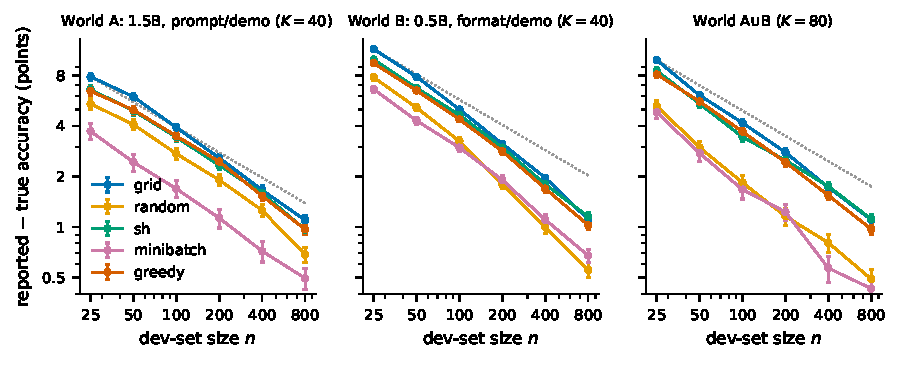
\includegraphics[width=\textwidth]{figs/gap_vs_n.pdf}
\caption{Reported (dev-set) minus true accuracy of the selected configuration against dev-set size, per optimizer (mean over $R{=}2000$ episodes, 95\% CI). Dotted: $n^{-1/2}$ reference through the exhaustive-search point at $n{=}25$.}\label{fig:gap}\end{figure*}
\textbf{Sizeable and slowly shrinking.} With exhaustive search over $K{=}40$ configurations and a dev set of $n{=}100$ questions the reported accuracy exceeds the true accuracy of the deployed configuration by $3.9$ (A), $5.0$ (B) and $4.2$ (A$\cup$B) points, i.e.\ 13\%, 33\% and 18\% relative (\cref{fig:gap}, \cref{tab:gap}); at $n{=}400$ it is still $1.7$, $2.0$, $1.7$. The decay is $n^{-0.57\dots-0.64}$ (log-log slope over $n\le400$), not faster than the $n^{-1/2}$ of \cref{prop:opt}. The overshoot is not merely a small bias: at $n{=}100$ the reported score exceeds the true accuracy of the \emph{best} configuration in the whole search space in 74\%, 83\% and 75\% of episodes (74--90\% over all five worlds), and the 95\% Wilson interval that one would attach to a fixed configuration covers the deployed configuration's accuracy only 88\%, 74\% and 86\% of the time (74--88\% over five worlds). \textbf{All optimizers inflate}, in proportion to how much they look at the dev set: minibatch (MIPRO-like) search and random-8 have the smallest gaps ($1.7/3.0/1.7$ and $2.7/3.2/1.8$ at $n{=}100$) and exhaustive search the largest. \cref{fig:effort} shows this dose--response directly: across optimizer settings the gap grows with the number of full-dev-set passes while the regret (how far $\theta_{\khat}$ is below the best configuration) improves by only $0.4$ points (A) and $2.4$ points (B) between a single configuration and the full grid, while the gap grows by $4$--$5$ points; much of the extra search effort buys optimism rather than accuracy (in A$\cup$B the gain in regret is large only for the first few configurations).
\begin{table}[t]
\caption{Reported $-$ true accuracy (points, mean $\pm$ 95\% CI) by optimizer and dev-set size $n$.}\label{tab:gap}
\centering\scriptsize\setlength{\tabcolsep}{3pt}
\begin{tabular}{lrrrr}\toprule
 & $n{=}50$ & 100 & 200 & 400 \\\midrule
\multicolumn{5}{l}{\emph{A: Qwen2.5-1.5B, prompt/demo grid ($K{=}40$)}} \\
Exhaustive & 6.0$\pm$0.3 & 3.9$\pm$0.2 & 2.6$\pm$0.1 & 1.7$\pm$0.1 \\
Random-8 & 4.1$\pm$0.3 & 2.7$\pm$0.2 & 1.9$\pm$0.1 & 1.3$\pm$0.1 \\
Succ. halving & 4.9$\pm$0.3 & 3.4$\pm$0.2 & 2.3$\pm$0.1 & 1.6$\pm$0.1 \\
Minibatch (MIPRO-like) & 2.4$\pm$0.3 & 1.7$\pm$0.2 & 1.1$\pm$0.1 & 0.7$\pm$0.1 \\
Greedy coord. & 5.0$\pm$0.3 & 3.5$\pm$0.2 & 2.5$\pm$0.1 & 1.5$\pm$0.1 \\
\multicolumn{5}{l}{\emph{B: Qwen2.5-0.5B, format/demo grid ($K{=}40$)}} \\
Exhaustive & 7.8$\pm$0.2 & 5.0$\pm$0.1 & 3.1$\pm$0.1 & 2.0$\pm$0.1 \\
Random-8 & 5.1$\pm$0.2 & 3.2$\pm$0.1 & 1.8$\pm$0.1 & 1.0$\pm$0.1 \\
Succ. halving & 6.7$\pm$0.2 & 4.6$\pm$0.1 & 3.0$\pm$0.1 & 1.8$\pm$0.1 \\
Minibatch (MIPRO-like) & 4.3$\pm$0.2 & 3.0$\pm$0.2 & 1.9$\pm$0.1 & 1.1$\pm$0.1 \\
Greedy coord. & 6.5$\pm$0.2 & 4.4$\pm$0.1 & 2.8$\pm$0.1 & 1.7$\pm$0.1 \\
\multicolumn{5}{l}{\emph{A$\cup$B: union ($K{=}80$)}} \\
Exhaustive & 6.1$\pm$0.3 & 4.2$\pm$0.2 & 2.8$\pm$0.1 & 1.7$\pm$0.1 \\
Random-8 & 3.0$\pm$0.3 & 1.8$\pm$0.2 & 1.2$\pm$0.1 & 0.8$\pm$0.1 \\
Succ. halving & 5.4$\pm$0.3 & 3.4$\pm$0.2 & 2.5$\pm$0.1 & 1.7$\pm$0.1 \\
Minibatch (MIPRO-like) & 2.7$\pm$0.3 & 1.7$\pm$0.2 & 1.2$\pm$0.1 & 0.6$\pm$0.1 \\
Greedy coord. & 5.6$\pm$0.3 & 3.7$\pm$0.2 & 2.4$\pm$0.1 & 1.5$\pm$0.1 \\
\bottomrule
\end{tabular}

\end{table}
\begin{figure*}[t]\centering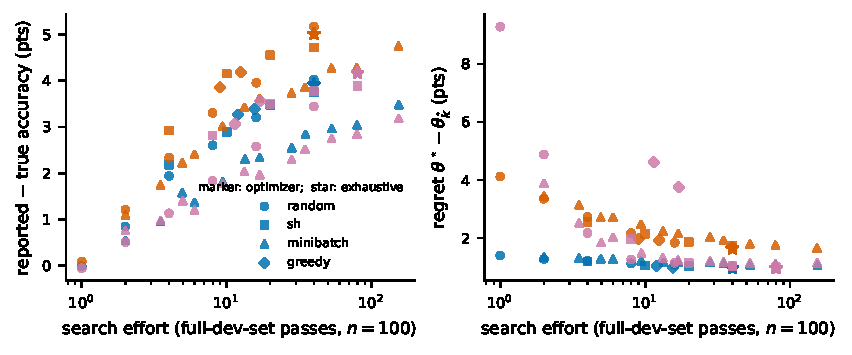
\includegraphics[width=.92\textwidth]{figs/search_effort.pdf}
\caption{Search effort vs.\ optimism (left) and regret (right), $n{=}100$; colours: worlds (blue A, orange B, pink A$\cup$B), markers: optimizer settings (random $B\in\{1,\dots,40\}$, SH budget, minibatch trials $\times$ minibatch size, greedy); stars: exhaustive.}\label{fig:effort}\end{figure*}

\subsection{What drives the gap}
\begin{figure*}[t]\centering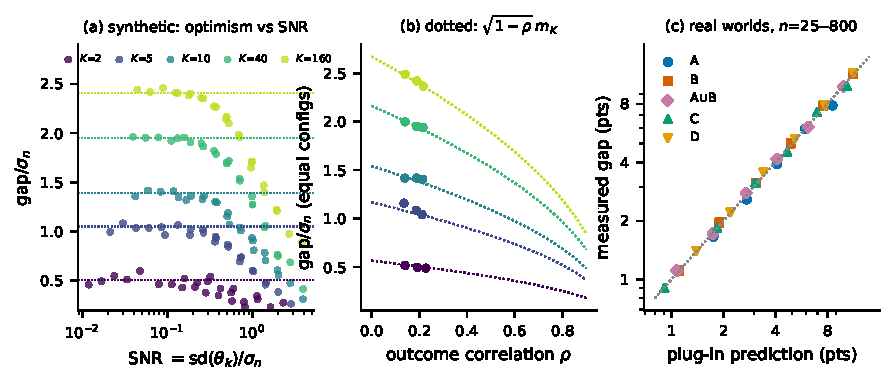
\includegraphics[width=\textwidth]{figs/theory_check.pdf}
\caption{(a,b) Synthetic worlds: optimism in units of $\sigma_n$ depends on the number of configurations $K$, their outcome correlation $\rho$, and the signal-to-noise ratio $\mathrm{sd}(\theta_k)/\sigma_n$; dotted: $\sqrt{1-\rho}\,m_K$ of \cref{prop:opt}(c). (c) Real worlds: Gaussian plug-in prediction (dev means $\sim N(\theta,\mathrm{Cov}(Y)/n)$, true $\theta$, Cov from the pool) vs.\ measured optimism of exhaustive search, all $n$.}\label{fig:theory}\end{figure*}
\cref{fig:theory}(a,b) confirm \cref{prop:opt}(c) on synthetic worlds: for equally good configurations the normalised optimism equals $\sqrt{1-\rho}\,m_K$ to within the plotting resolution, and it falls with $\mathrm{SNR}=\mathrm{sd}(\theta_k)/\sigma_n$ once the best configuration becomes identifiable. On the real worlds a Gaussian plug-in that uses the pool's $\theta$ and outcome covariance predicts the measured optimism of exhaustive search within $9.2\%$ (mean $2.6\%$) for all 30 (world, $n$) cells of the five worlds (\cref{fig:theory}c; the figure marks A, B, A$\cup$B, C, D), so the mechanism is the maximum of correlated, approximately Gaussian estimation errors. Practical consequences: (i) \emph{number of effectively distinct configurations}, not nominal $K$, matters---world A has $\bar\rho{=}0.79$ and a gap of $3.9$ points, world B ($\bar\rho{=}0.33$) $5.0$ at lower accuracy; (ii) the gap is governed by $\sigma_n=\sqrt{p(1-p)/n}$, so it is largest relative to accuracy for hard benchmarks and small $n$; (iii) \cref{fig:ksweep} (appendix) shows that the gap grows roughly like $\sqrt{\ln K}$ with the number of configurations searched.

\subsection{Effect on conclusions drawn from reported scores}
\begin{figure*}[t]\centering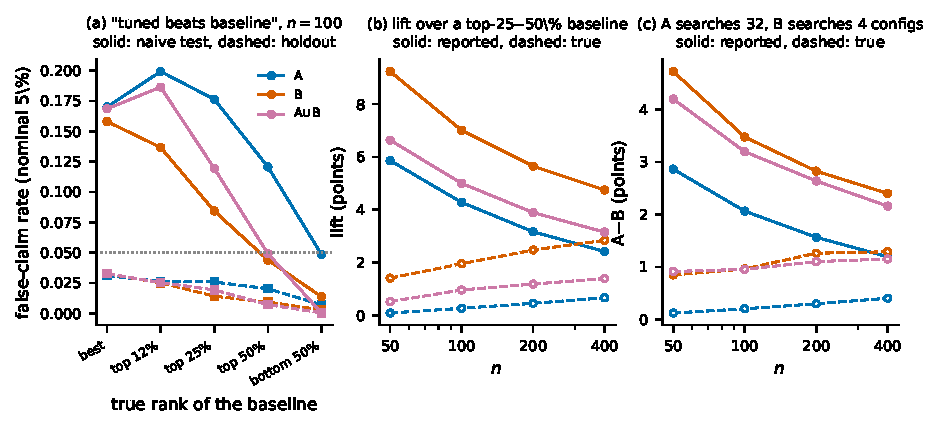
\includegraphics[width=\textwidth]{figs/conclusions.pdf}
\caption{Consequences. (a) A paired one-sided test (nominal 5\%) that the tuned system beats a baseline configuration, as a function of the baseline's true rank in the space: fraction of \emph{false} claims (claim made while the true lift is $\le0$) with the naive test (solid) and with a 50/50 holdout (dashed). (b) Reported vs.\ true lift over a baseline from the 25--50\% quantile. (c) System A tuned over 32 configurations vs.\ system B tuned over 4 (disjoint, random); reported vs.\ true difference.}\label{fig:concl}\end{figure*}
\textbf{Lifts over a baseline.} A natural claim is ``automatic tuning improved accuracy by $\delta$ over the baseline prompt''. If the baseline is already a good configuration (top 12\% of the space), the one-sided paired test on the dev set declares a significant improvement in $19$/$14$/$18\%$ of episodes at $n{=}100$ (A/B/A$\cup$B) although tuning cannot help; the 50/50 holdout test errs in $3\%$. For a mid-ranked baseline (true rank in the top 25--50\%) the reported lift at $n{=}100$ is $4.3/7.0/5.0$ points versus true lifts of $0.3/2.0/1.0$ (\cref{tab:concl}, \cref{fig:concl}b)---in world A tuning delivers nothing measurable although the average episode ``finds'' a multi-point gain. \textbf{Comparing systems tuned with different budgets.} If system A searches 32 configurations and B searches 4 on the same dev set, the reported advantage of A is $2.1/3.5/3.2$ points versus a true advantage of $0.2/1.0/1.0$ (A/B/A$\cup$B, $n{=}100$): a 3--10$\times$ inflation (\cref{prop:cmp}); the holdout comparison is unbiased for the selected pair ($0.0/0.9/0.9$).
\begin{table}[t]
\caption{Claims at $n$ questions ($K_A{=}32$ vs $K_B{=}4$ in the last columns). False-claim rate: baseline in the top 12\% of the space, nominal 5\%. Lift: baseline of true rank 11--20 of $K$ (top 25--50\%), reported / true (points); `holdout lift' is the 50/50 holdout estimate. A$-$B: reported / true (points) and holdout estimate.}\label{tab:concl}
\centering\scriptsize\setlength{\tabcolsep}{2.5pt}
\begin{tabular}{rrrrrrr}\toprule
$n$ & false claim & (holdout) & lift & holdout lift & A$-$B & (holdout) \\\midrule
\multicolumn{7}{l}{\emph{A: Qwen2.5-1.5B, prompt/demo grid ($K{=}40$)}} \\
50 & 0.22 & 0.02 & 5.9 / 0.1 & -0.1 & 2.9 / 0.1 & -0.1 \\
100 & 0.19 & 0.03 & 4.3 / 0.3 & 0.1 & 2.1 / 0.2 & 0.0 \\
200 & 0.14 & 0.02 & 3.2 / 0.5 & 0.3 & 1.6 / 0.3 & 0.2 \\
400 & 0.10 & 0.02 & 2.4 / 0.7 & 0.4 & 1.2 / 0.4 & 0.3 \\
\multicolumn{7}{l}{\emph{B: Qwen2.5-0.5B, format/demo grid ($K{=}40$)}} \\
50 & 0.18 & 0.02 & 9.2 / 1.4 & 0.9 & 4.7 / 0.8 & 0.7 \\
100 & 0.14 & 0.03 & 7.0 / 2.0 & 1.4 & 3.5 / 1.0 & 0.9 \\
200 & 0.11 & 0.02 & 5.6 / 2.5 & 2.0 & 2.8 / 1.3 & 1.0 \\
400 & 0.07 & 0.01 & 4.7 / 2.8 & 2.4 & 2.4 / 1.3 & 1.2 \\
\multicolumn{7}{l}{\emph{A$\cup$B: union ($K{=}80$)}} \\
50 & 0.20 & 0.02 & 6.6 / 0.5 & -0.8 & 4.2 / 0.9 & 0.6 \\
100 & 0.18 & 0.03 & 5.0 / 1.0 & 0.5 & 3.2 / 1.0 & 0.9 \\
200 & 0.13 & 0.02 & 3.9 / 1.2 & 1.0 & 2.6 / 1.1 & 1.0 \\
400 & 0.10 & 0.02 & 3.2 / 1.4 & 1.2 & 2.2 / 1.1 & 1.0 \\
\bottomrule
\end{tabular}

\end{table}

\subsection{Reporting protocols}
\begin{table*}[t]
\caption{Reporting protocols, exhaustive search, $n{=}100$, $R{=}2000$ episodes. Bias and RMSE of the estimate of the deployed configuration's true accuracy (points; for holdout the target is the accuracy of the holdout-selected configuration), coverage and mean width (points) of the nominal 95\% interval; s.e.\ of bias $\le0.4$, of coverage $\le1$ point. Max-$t$ is centred at the naive score; empirical Bayes uses the recentred interval.}\label{tab:proto}
\centering\scriptsize\setlength{\tabcolsep}{4pt}
\begin{tabular}{lrrrr}\toprule
Protocol & bias & RMSE & coverage & width \\\midrule
\multicolumn{5}{l}{\emph{A: Qwen2.5-1.5B, prompt/demo grid ($K{=}40$)}} \\
Naive (dev score) & +3.9 & 5.8 & 0.88 & 18.3 \\
Holdout split (50/50) & +0.0 & 6.4 & 0.95 & 24.6 \\
5-fold cross-fit & -0.2 & 5.1 & -- & -- \\
Replay bootstrap (opt.) & +1.1 & 4.6 & -- & -- \\
Replay bootstrap (.632) & +1.3 & 4.6 & -- & -- \\
Empirical Bayes & +0.1 & 4.3 & 0.96 & 18.7 \\
Max-t simultaneous & +3.9 & 5.8 & 0.98 & 25.6 \\
Conditional (winner) & -8.7 & 18.3 & 0.72 & 21.9 \\
Ladder ($n^{-1/2}$) & +0.2 & 5.0 & -- & -- \\
\multicolumn{5}{l}{\emph{B: Qwen2.5-0.5B, format/demo grid ($K{=}40$)}} \\
Naive (dev score) & +5.0 & 5.9 & 0.74 & 16.1 \\
Holdout split (50/50) & +0.1 & 5.3 & 0.95 & 20.3 \\
5-fold cross-fit & -0.3 & 4.8 & -- & -- \\
Replay bootstrap (opt.) & +1.0 & 3.7 & -- & -- \\
Replay bootstrap (.632) & +1.5 & 3.7 & -- & -- \\
Empirical Bayes & -0.3 & 3.3 & 0.98 & 15.6 \\
Max-t simultaneous & +5.0 & 5.9 & 1.00 & 25.4 \\
Conditional (winner) & -3.1 & 9.6 & 0.82 & 22.1 \\
Ladder ($n^{-1/2}$) & +1.9 & 4.5 & -- & -- \\
\multicolumn{5}{l}{\emph{A$\cup$B: union ($K{=}80$)}} \\
Naive (dev score) & +4.2 & 6.0 & 0.86 & 18.4 \\
Holdout split (50/50) & -0.1 & 6.5 & 0.95 & 24.5 \\
5-fold cross-fit & +0.1 & 5.2 & -- & -- \\
Replay bootstrap (opt.) & +1.2 & 4.8 & -- & -- \\
Replay bootstrap (.632) & +1.3 & 4.7 & -- & -- \\
Empirical Bayes & +2.3 & 5.2 & 0.88 & 16.0 \\
Max-t simultaneous & +4.2 & 6.0 & 0.99 & 30.0 \\
Conditional (winner) & -7.8 & 17.8 & 0.73 & 22.5 \\
Ladder ($n^{-1/2}$) & +0.7 & 5.2 & -- & -- \\
\bottomrule
\end{tabular}

\end{table*}
\begin{figure}[t]\centering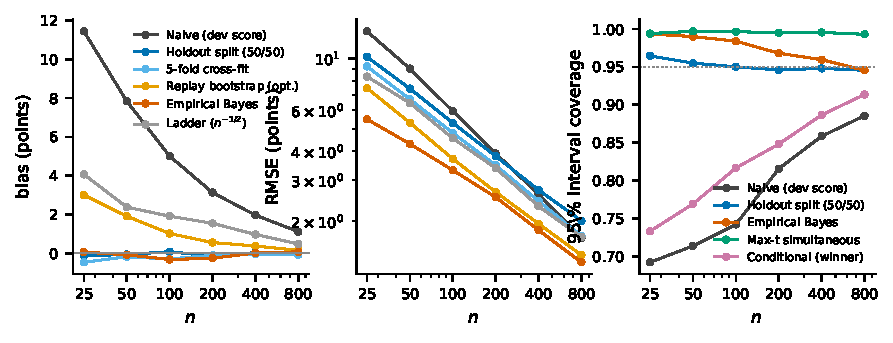
\includegraphics[width=\columnwidth]{figs/protocols_b05.pdf}
\caption{Bias, RMSE and coverage of the protocols against $n$, exhaustive search, world B (other worlds in \cref{fig:protocols}).}\label{fig:proto_b}\end{figure}
\textbf{Sample splitting} (P2) is unbiased with exact 95\% coverage in every world, but is not accurate: its RMSE is $5.3$--$6.5$ points at $n{=}100$ (no better than the naive score in A and A$\cup$B, because discarding half of the questions doubles the sampling variance of the score), its interval is wider than the naive one ($20$--$25$ vs.\ $16$--$18$ points), and it deploys a worse configuration ($-0.16/-0.55/-0.45$ points at $f{=}0.5$; up to $-1.3$ at $f{=}0.3$; \cref{tab:split}). Cross-fitting (P3) has low bias for the procedure but cannot attach an interval to the specific $\khat$. The \textbf{search-replay bootstrap} (P4) removes $70$--$80\%$ of the optimism for exhaustive search (at $n{=}100$ residual bias $+1.1/+1.0/+1.2$ vs.\ $+3.9/+5.0/+4.2$; RMSE $4.6/3.7/4.8$, lower than splitting). The \textbf{empirical-Bayes} correction (P5) is the most accurate dev-set-only method when configurations look exchangeable (A: bias $+0.1$, RMSE $4.3$; B: $-0.3$, $3.3$; recentred interval coverage $0.96$/$0.98$ at the width of the naive interval), but it \emph{fails when the prior is not roughly normal}: in A$\cup$B (two quality clusters) its bias is $+2.3$ and coverage $0.88$, and it requires scoring all configurations on all of $D$. \textbf{Max-$t$} (P6) is conservative but always valid for exhaustive/random search (coverage $\ge0.98$; width $25$--$30$ points vs.\ $16$--$18$ for naive); its point estimate is the biased naive score. The \textbf{conditional winner} interval (P7) is poorly calibrated for discrete accuracies (coverage $0.72$--$0.82$, RMSE $9.6$--$18$ points) although our implementation attains $95.4\%$ coverage on continuous Gaussian data (\texttt{code/check\_cond.py}), i.e.\ the Gaussian/ties approximation, not the principle, is at fault. The \textbf{Ladder} (P8) is nearly unbiased only where nothing is really better (A) because it rarely moves off its starting configuration; in B it deploys $1.1$ points less accuracy than exhaustive search and still reports $+1.9$ too high. Appendix tables repeat the comparison for all optimizers (replay bootstrap and, heuristically, empirical Bayes remain reasonably accurate for minibatch and greedy search) and $n$.

\begin{table}[t]
\caption{Cost and accuracy of sample splitting, exhaustive search, $n{=}100$. `cost' = loss in true accuracy of the deployed configuration relative to selecting with all $n$ (points).}\label{tab:split}
\centering\scriptsize\setlength{\tabcolsep}{3pt}
\begin{tabular}{lrrrrr}\toprule
Protocol & cost & bias & RMSE & cover. & width \\\midrule
\multicolumn{6}{l}{\emph{A: Qwen2.5-1.5B, prompt/demo grid ($K{=}40$)}} \\
no split (naive) & 0.0 & +3.9 & 5.8 & 0.88 & 18.3 \\
select on 30\% / report on 70\% & 0.27 & -0.1 & 5.4 & 0.96 & 21.0 \\
select on 50\% / report on 50\% & 0.16 & +0.0 & 6.4 & 0.95 & 24.6 \\
select on 70\% / report on 30\% & 0.09 & +0.1 & 8.4 & 0.95 & 31.0 \\
\multicolumn{6}{l}{\emph{B: Qwen2.5-0.5B, format/demo grid ($K{=}40$)}} \\
no split (naive) & 0.0 & +5.0 & 5.9 & 0.74 & 16.1 \\
select on 30\% / report on 70\% & 1.00 & -0.0 & 4.6 & 0.94 & 17.0 \\
select on 50\% / report on 50\% & 0.55 & +0.1 & 5.3 & 0.95 & 20.3 \\
select on 70\% / report on 30\% & 0.32 & -0.1 & 6.8 & 0.95 & 25.8 \\
\multicolumn{6}{l}{\emph{A$\cup$B: union ($K{=}80$)}} \\
no split (naive) & 0.0 & +4.2 & 6.0 & 0.86 & 18.4 \\
select on 30\% / report on 70\% & 1.26 & +0.0 & 5.5 & 0.95 & 20.8 \\
select on 50\% / report on 50\% & 0.45 & -0.1 & 6.5 & 0.95 & 24.5 \\
select on 70\% / report on 30\% & 0.16 & -0.2 & 8.3 & 0.95 & 30.9 \\
\bottomrule
\end{tabular}

\end{table}

\section{Discussion and limitations}
\label{sec:discussion}
\textbf{What the results say.} Reporting the score of an automatically tuned configuration on the questions that guided the search overstates its accuracy on new questions by an amount that is large when the dev set is the size typical for tuning ($n\lesssim 200$), shrinks only slowly with $n$, and depends on the search-space diversity and the signal-to-noise ratio in the way \cref{prop:opt} predicts. The inflation spills over to the conclusions drawn from the numbers: lifts over a baseline, significance of a paired test, and comparisons between systems tuned with different budgets. Sample splitting makes the report unbiased for any optimizer at the cost of selection quality and of interval width; model-based corrections that exploit the paired structure of the outcomes (empirical Bayes, replay bootstrap) are markedly more accurate when every configuration is scored on the same questions, but their validity rests on assumptions that hold only approximately.

\textbf{Practical recommendations.} (1) Report the held-out score of the deployed configuration, with the number of configurations/trials searched and $n$; a 50/50 split is a reasonable default (\cref{tab:split}: selecting on 30\% gives a more precise report in every world but loses up to 1.3 points of deployed accuracy, selecting on 70\% a much noisier report). (2) If all questions must be used for search, report a search-aware estimate (empirical Bayes or replay bootstrap) \emph{together with} the naive score, and a simultaneous lower bound if a guarantee is needed. (3) Do not compare systems tuned with unequal budgets on a shared dev set without correcting for the budget. (4) Treat dev-set lifts smaller than the optimism predicted by \cref{prop:opt} (about $\sigma_n\sqrt{1-\rho}\,m_K$ for equally good configurations) as unresolved.

\textbf{Limitations.} \emph{Simulated search over cached configurations.} Our optimizers replay the search logic of DSPy/MIPRO/best-arm-identification methods on discrete, pre-computed spaces of 40--80 configurations; we did not run those tools end-to-end (their LLM-proposed instructions and bootstrapped demonstrations are open-ended spaces and need generation-based evaluation that was beyond our CPU budget). The qualitative mechanism does not depend on this, but absolute gaps for those tools could differ. \emph{Models and task.} The worlds use Qwen2.5-0.5B/1.5B-Instruct and SmolLM2-1.7B-Instruct (three models, two families) with log-probability answer scoring on a random sample of MMLU-Pro questions of $\le 200$ tokens (about 65\% of the benchmark; long law/history items are under-represented), without chain-of-thought and with deterministic decoding; prompt effects on larger models or generative reasoning pipelines may be larger or smaller, which by \cref{prop:opt} moves the SNR and hence the gap. \emph{Finite pool.} Truth is defined on a pool of $N{=}750$ questions per world ($N{=}450$ for world D); the benchmark is the empirical distribution of the pool, and results for $n$ close to $N$ should be read with that in mind (the without-replacement check in \cref{tab:norepl} covers $n\le 200$; bootstrapping the pool gives a 95\% range of about $\pm0.5$--$0.7$ points for the gap at $n{=}100$, \cref{tab:poolboot}). \emph{Protocols.} Empirical Bayes assumes exchangeable, roughly normal true accuracies and a fully evaluated configuration set; its simple interval loses coverage at large $n$ and for adaptive optimizers; max-$t$ and the conditional method were applied to exhaustive/random search only (applying them to adaptively visited sets is heuristic and, for max-$t$ with few visited configurations, fails); the conditional method uses a Gaussian approximation to discrete accuracies and is poorly calibrated here. We did not evaluate the reusable holdout or differentially private mechanisms beyond the Ladder, nor distribution shift between benchmark and deployment, question clustering, or label noise.


\section*{Impact Statement}
This paper studies how benchmark scores of automatically tuned LLM systems should be interpreted and reported. We expect a positive effect on scientific practice (less over-claiming, fairer comparisons between systems tuned with different budgets). We see no direct negative societal consequences; one risk is that the more conservative intervals we advocate may be read as a general reason to distrust any tuned system, whereas our results are specific to the regimes studied. All experiments use public data and small open-weight models on CPU.


\bibliography{refs}
\bibliographystyle{icml2026}

\appendix
\onecolumn
\raggedbottom
\section{Implementation details}
\label{app:impl}
\textbf{Scoring.} Every configuration is a chat (ChatML) or raw prompt; the model's next-token logits at the position after the answer prefix (``The answer is ('' or ``Answer:'') are restricted to the letters A--J that exist for the question, and the arg-max letter is the prediction. The shared prefix (system prompt and demonstrations) is computed once and its key/value cache re-used for all questions (verified to reproduce uncached logits up to fp16 storage rounding). fp32 inference on 4 CPU cores; no sampling.
\textbf{World A} ($K{=}40$): instruction $\in$ \{none (template default system prompt), ``You are a helpful assistant.'', ``Answer the following multiple-choice question. Respond with the letter of the correct option.'', ``You are a world-class expert across all academic disciplines. Choose the single best answer.'', ``Read the question carefully, eliminate options that are clearly wrong, and select the most likely correct answer.'', ``The following are multiple choice questions from a difficult university-level exam. Be precise.'', ``Be careful: many questions look easy but contain subtle traps. Think about what the question is really asking before choosing.'', ``Reply with only the letter of the best option.''\} $\times$ demonstration set $\in$ \{zero-shot, four random 3-shot sets from the 70 MMLU-Pro validation questions\}; demonstrations are answer-only chat turns.
\textbf{World B} ($K{=}40$): format $\in$ \{chat with ``Options:'' block and an instruction line; raw text (no chat template, ``Question: \dots Answer:''); chat with ``(A)''-style options and ``Answer:'' prefix; chat without the instruction line; chat with options before the question\} $\times$ demonstrations $\in$ \{zero-shot, 3 random, 3 validation questions that all have answer ``A'', 8 random\} $\times$ instruction $\in$ \{none, ``world-class expert''\}.
\textbf{Pool.} Questions whose ``question + options'' text has at most 200 Qwen tokens (about $7{,}900$ of $12{,}032$ test questions); a seeded permutation (seed 12345) and the first 750 (world D: 450) are used, with the same Qwen tokenizer defining the pool for every model. Category composition of the eligible set: math 15\%, physics 12\%, other 10\%, economics 9\%, health 8\%, \dots, law 2\%, history 2\%.
\textbf{Optimizers} (code: \texttt{code/sim\_lib.py}). \emph{Exhaustive}: all $K$ configurations on all $n$ questions. \emph{Random-8}: 8 random configurations. \emph{SH}: successive halving over questions, total budget $0.5Kn$ (config, question) evaluations, $\lceil\log_2 K\rceil$ rounds, final winner re-scored on all of $D$ for the report. \emph{Minibatch}: 30 trials; each proposes a uniformly random configuration (prob.\ 0.5) or a one-factor neighbour of the current best-by-running-mean, scores it on a random minibatch of $0.25n$ questions, and every 10 trials the incumbent is scored on all of $D$; the final choice is the best full-$D$ score. \emph{Greedy}: from a random start, up to 3 sweeps of coordinate ascent over the factor axes with full-$D$ scores. Ties are broken uniformly at random.
\textbf{Protocol details} (\texttt{code/sim\_lib.py}, \texttt{code/episodes.py}). Wilson intervals; holdout fractions $f\in\{0.3,0.5,0.7\}$; 5-fold cross-fit; replay bootstrap $B{=}100$; max-$t$ uses 1000 Gaussian multipliers and studentised errors with $\hat\sigma_k=\sqrt{\hat p_k(1-\hat p_k)}$ (floored at $1/(2\sqrt n)$); empirical Bayes: $\theta_k=g+d_k$, $d_k\sim N(0,\tau^2)$, centred paired covariance $\hat S/n$, $\hat\tau^2=\max\{0,\|\hat d\|^2/(m-1)-\mathrm{tr}(P\hat SP)/(m-1)\}$, posterior mean $\bar{\bar y}+\hat B\hat d_{\hat k}$ with $\hat B=\hat\tau^2/(\hat\tau^2+v_{\hat k})$; the reported interval is est.\ $\pm1.96\sqrt{u+v_{\hat k}}$ with $u$ the sampling variance of the grand mean (a ``posterior'' interval with $\hat B v_{\hat k}$ instead of $v_{\hat k}$ under-covers: 0.85--0.95 in our worlds); conditional inference: truncation limits from the polyhedron $\{\bar Y_k\ge\bar Y_j\,\forall j\}$ with the empirical covariance, exact ties replaced by a uniform jitter of width $1/n$; Ladder with step $\eta=n^{-1/2}$ ($n^{-1/3}$ variant also computed, deploys much worse configurations: $-7.0$ points in A$\cup$B at $n{=}100$). Max-$t$, empirical Bayes and conditional inference are applied to the set of fully evaluated configurations; for adaptive optimizers (greedy, minibatch) this is heuristic, and for SH it is undefined (one fully evaluated configuration).
\textbf{Synthetic worlds} (\texttt{code/worlds.py::synth\_world}): $Y_{ki}\sim\mathrm{Bernoulli}(\mathrm{sigmoid}(\mu+d_i+c_k+s\,e_{ki}))$ with $d_i\sim N(0,1.2^2)$ (difficulty), $c_k\sim N(0,\tau^2)$ (configuration effect), $e_{ki}\sim N(0,1)$ (interaction, controls $\rho$), $N=20000$; sweep $K\in\{2,5,10,40,160\}$, $\tau\in\{0,.05,.1,.2,.4\}$, $s\in\{.3,.8,1.5\}$, $n\in\{50,\dots,800\}$, 400 episodes per cell.

\section{Additional results}
\label{app:extra}
\begin{figure}[H]\centering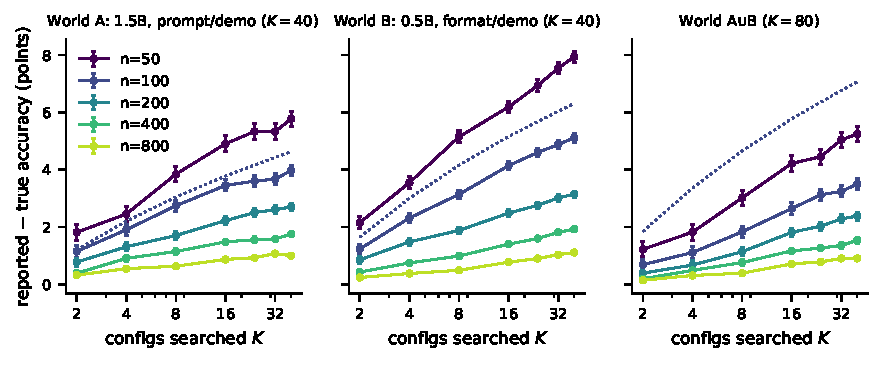
\includegraphics[width=.95\textwidth]{figs/gap_vs_K.pdf}
\caption{Optimism of exhaustive search over a random subset of $K$ of the configurations of each world, by dev-set size (95\% CI; 1000 episodes per point). Dotted ($n{=}100$): equal-quality prediction $\sigma_n\sqrt{1-\bar\rho}\,m_K$, an upper reference when configurations differ in quality.}\label{fig:ksweep}\end{figure}
\begin{figure}[H]\centering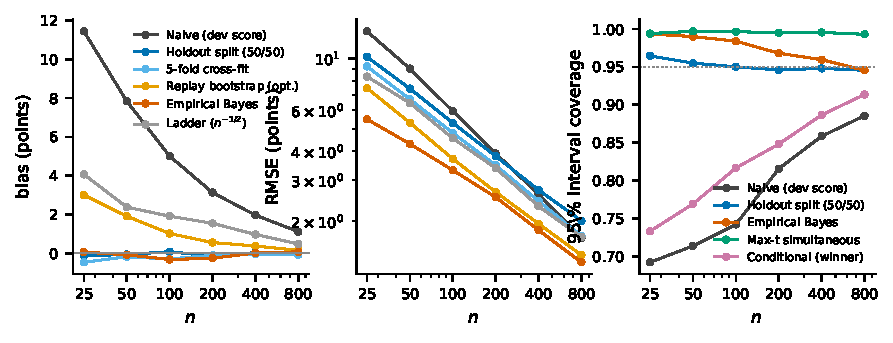
\includegraphics[width=.75\textwidth]{figs/protocols_b05.pdf}\\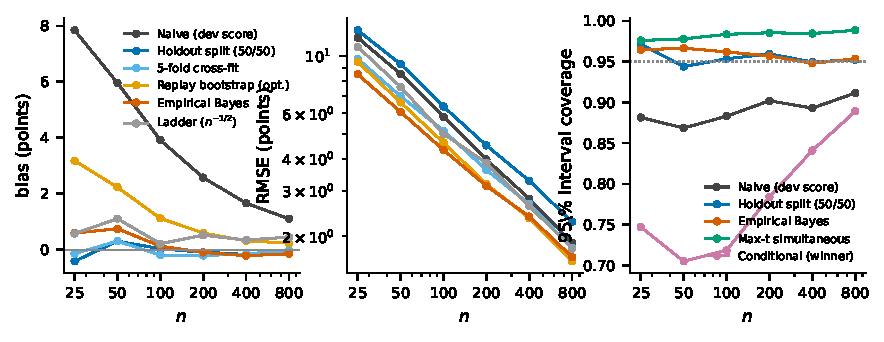
\includegraphics[width=.75\textwidth]{figs/protocols_q15.pdf}\\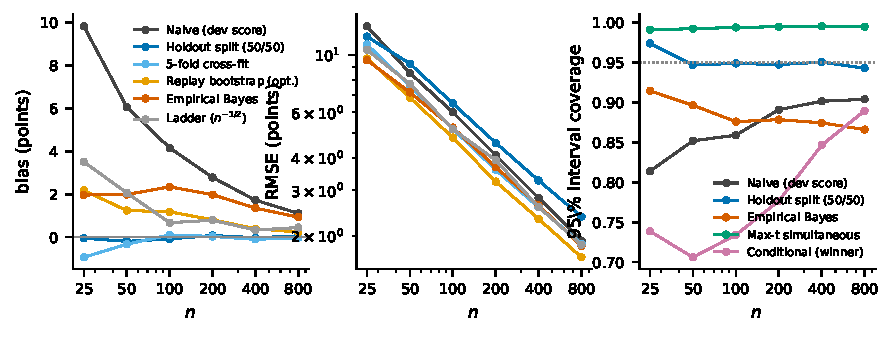
\includegraphics[width=.75\textwidth]{figs/protocols_mix.pdf}
\caption{Bias, RMSE and interval coverage of the protocols against $n$ for exhaustive search in world B (top), A (middle), A$\cup$B (bottom); worlds C and D: \cref{tab:proto_extra}.}\label{fig:protocols}\end{figure}
\begin{table}[H]
\caption{Protocols for every optimizer, $n{=}100$ (points; coverage as fraction). Bias and RMSE of the naive score; RMSE of the 50/50 holdout; bias and RMSE of the replay bootstrap; bias, RMSE and coverage of empirical Bayes (heuristic for greedy/minibatch, undefined for SH).}\label{tab:allopt}
\centering\scriptsize\setlength{\tabcolsep}{4pt}
\begin{tabular}{lrrrrrrrr}\toprule
\multicolumn{1}{l}{} & \multicolumn{2}{c}{naive} & hold. & \multicolumn{2}{c}{replay boot.} & \multicolumn{3}{c}{emp.\ Bayes} \\
 & bias & RMSE & RMSE & bias & RMSE & bias & RMSE & cov. \\\midrule
\multicolumn{9}{l}{\emph{A: Qwen2.5-1.5B, prompt/demo grid ($K{=}40$)}} \\
Exhaustive & 3.9 & 5.8 & 6.4 & 1.1 & 4.6 & 0.1 & 4.3 & 0.96 \\
Random-8 & 2.7 & 5.2 & 6.7 & 0.8 & 4.6 & 0.4 & 4.4 & 0.95 \\
Succ. halving & 3.4 & 5.6 & 6.7 & 0.9 & 4.6 & -- & -- & -- \\
Minibatch (MIPRO-like) & 1.7 & 4.9 & 6.5 & 0.3 & 4.6 & 0.8 & 4.3 & 0.97 \\
Greedy coord. & 3.5 & 5.7 & 6.5 & 1.1 & 4.8 & 1.0 & 4.7 & 0.95 \\
\multicolumn{9}{l}{\emph{B: Qwen2.5-0.5B, format/demo grid ($K{=}40$)}} \\
Exhaustive & 5.0 & 5.9 & 5.3 & 1.0 & 3.7 & -0.3 & 3.3 & 0.98 \\
Random-8 & 3.2 & 4.7 & 5.4 & 0.6 & 3.5 & -0.3 & 3.4 & 0.97 \\
Succ. halving & 4.6 & 5.7 & 5.3 & 1.0 & 3.7 & -- & -- & -- \\
Minibatch (MIPRO-like) & 3.0 & 4.7 & 5.2 & 0.4 & 3.7 & 1.4 & 3.6 & 0.99 \\
Greedy coord. & 4.4 & 5.5 & 5.3 & 1.1 & 3.7 & 1.0 & 3.6 & 0.96 \\
\multicolumn{9}{l}{\emph{A$\cup$B: union ($K{=}80$)}} \\
Exhaustive & 4.2 & 6.0 & 6.5 & 1.2 & 4.8 & 2.3 & 5.2 & 0.88 \\
Random-8 & 1.8 & 4.9 & 6.6 & 0.3 & 4.7 & 0.2 & 4.9 & 0.91 \\
Succ. halving & 3.4 & 5.6 & 6.6 & 0.6 & 4.6 & -- & -- & -- \\
Minibatch (MIPRO-like) & 1.7 & 4.9 & 6.6 & 0.2 & 4.8 & 0.9 & 4.7 & 0.97 \\
Greedy coord. & 3.7 & 5.5 & 6.4 & 1.0 & 4.3 & 2.0 & 4.8 & 0.92 \\
\bottomrule
\end{tabular}

\end{table}
\begin{table}[H]
\caption{Draws without replacement (dev set $D$ of $n$ distinct pool questions): optimism relative to the pool accuracy and relative to the accuracy on the \emph{remaining} pool questions (fresh), compared with the i.i.d.\ design of the main text (points).}\label{tab:norepl}
\centering\scriptsize\setlength{\tabcolsep}{4pt}
\begin{tabular}{lrrr}\toprule
 & i.i.d.\ (main) & w/o repl., vs pool & w/o repl., vs fresh \\\midrule
\multicolumn{4}{l}{\emph{A: Qwen2.5-1.5B, prompt/demo grid ($K{=}40$)}} \\
Exhaustive, $n{=}50$ & 6.0 & 5.7 & 6.1$\pm$0.3 \\
Exhaustive, $n{=}100$ & 3.9 & 3.6 & 4.2$\pm$0.2 \\
Exhaustive, $n{=}200$ & 2.6 & 2.4 & 3.3$\pm$0.2 \\
Minibatch (MIPRO-like), $n{=}50$ & 2.4 & 2.3 & 2.5$\pm$0.3 \\
Minibatch (MIPRO-like), $n{=}100$ & 1.7 & 1.5 & 1.7$\pm$0.2 \\
Minibatch (MIPRO-like), $n{=}200$ & 1.1 & 0.8 & 1.1$\pm$0.2 \\
\multicolumn{4}{l}{\emph{B: Qwen2.5-0.5B, format/demo grid ($K{=}40$)}} \\
Exhaustive, $n{=}50$ & 7.8 & 7.3 & 7.8$\pm$0.2 \\
Exhaustive, $n{=}100$ & 5.0 & 4.5 & 5.2$\pm$0.2 \\
Exhaustive, $n{=}200$ & 3.1 & 2.5 & 3.4$\pm$0.1 \\
Minibatch (MIPRO-like), $n{=}50$ & 4.3 & 4.2 & 4.6$\pm$0.2 \\
Minibatch (MIPRO-like), $n{=}100$ & 3.0 & 2.5 & 2.9$\pm$0.2 \\
Minibatch (MIPRO-like), $n{=}200$ & 1.9 & 1.3 & 1.8$\pm$0.1 \\
\multicolumn{4}{l}{\emph{A$\cup$B: union ($K{=}80$)}} \\
Exhaustive, $n{=}50$ & 6.1 & 6.0 & 6.4$\pm$0.3 \\
Exhaustive, $n{=}100$ & 4.2 & 3.6 & 4.2$\pm$0.2 \\
Exhaustive, $n{=}200$ & 2.8 & 2.4 & 3.3$\pm$0.2 \\
Minibatch (MIPRO-like), $n{=}50$ & 2.7 & 2.5 & 2.7$\pm$0.3 \\
Minibatch (MIPRO-like), $n{=}100$ & 1.7 & 1.3 & 1.5$\pm$0.2 \\
Minibatch (MIPRO-like), $n{=}200$ & 1.2 & 0.8 & 1.1$\pm$0.2 \\
\bottomrule
\end{tabular}

\end{table}
\begin{table}[H]
\caption{Uncertainty from the finite pool: exhaustive-search optimism (points) in the main design (the actual 750-question pool) and over 200 bootstrap resamples of the pool (each a new world; 400 episodes each); the 95\% range is over worlds.}\label{tab:poolboot}
\centering\scriptsize\setlength{\tabcolsep}{4pt}
\begin{tabular}{lrrr}\toprule
world, $n$ & main design & pool-bootstrap mean & 95\% range \\\midrule
A, $n{=}50$ & 6.0 & 5.6 & 4.9--6.2 \\
A, $n{=}100$ & 3.9 & 3.8 & 3.3--4.3 \\
A, $n{=}400$ & 1.7 & 1.5 & 1.0--1.9 \\
B, $n{=}50$ & 7.8 & 7.7 & 7.0--8.4 \\
B, $n{=}100$ & 5.0 & 4.9 & 4.1--5.5 \\
B, $n{=}400$ & 2.0 & 1.7 & 1.0--2.3 \\
A$\cup$B, $n{=}50$ & 6.1 & 6.0 & 5.3--6.8 \\
A$\cup$B, $n{=}100$ & 4.2 & 3.8 & 3.2--4.3 \\
A$\cup$B, $n{=}400$ & 1.7 & 1.5 & 1.0--1.9 \\
\bottomrule
\end{tabular}

\end{table}
\begin{table}[H]
\caption{Gap and regret by optimizer setting, $n{=}100$ (the data behind \cref{fig:effort}); `effort' is the number of full-dev-set passes.}\label{tab:optsens}
\centering\scriptsize\setlength{\tabcolsep}{4pt}
\begin{tabular}{lrrr}\toprule
setting & effort & gap & regret \\\midrule
\multicolumn{4}{l}{\emph{A: Qwen2.5-1.5B, prompt/demo grid ($K{=}40$)}} \\
greedy sweeps: 1 & 12.0 & 3.3$\pm$0.2 & 1.0 \\
greedy sweeps: 3 & 15.6 & 3.4$\pm$0.2 & 1.0 \\
minibatch T: 10, bfrac: 0.1 & 2.0 & 0.6$\pm$0.2 & 1.3 \\
minibatch T: 10, bfrac: 0.25 & 3.5 & 1.0$\pm$0.2 & 1.3 \\
minibatch T: 30, bfrac: 0.1 & 4.9 & 1.6$\pm$0.2 & 1.3 \\
minibatch T: 10, bfrac: 0.5 & 6.0 & 1.4$\pm$0.2 & 1.3 \\
minibatch T: 30, bfrac: 0.25 & 9.4 & 1.8$\pm$0.2 & 1.2 \\
minibatch T: 100, bfrac: 0.1 & 13.4 & 2.3$\pm$0.2 & 1.2 \\
minibatch T: 30, bfrac: 0.5 & 16.9 & 2.3$\pm$0.2 & 1.2 \\
minibatch T: 100, bfrac: 0.25 & 28.1 & 2.5$\pm$0.2 & 1.2 \\
minibatch T: 300, bfrac: 0.1 & 35.0 & 2.8$\pm$0.2 & 1.1 \\
minibatch T: 100, bfrac: 0.5 & 53.0 & 3.0$\pm$0.2 & 1.1 \\
minibatch T: 300, bfrac: 0.25 & 79.6 & 3.0$\pm$0.2 & 1.1 \\
minibatch T: 300, bfrac: 0.5 & 154.2 & 3.5$\pm$0.2 & 1.1 \\
random B: 1 & 1.0 & -0.0$\pm$0.2 & 1.4 \\
random B: 2 & 2.0 & 0.8$\pm$0.2 & 1.3 \\
random B: 4 & 4.0 & 1.9$\pm$0.2 & 1.2 \\
random B: 8 & 8.0 & 2.6$\pm$0.2 & 1.1 \\
random B: 16 & 16.0 & 3.2$\pm$0.2 & 1.1 \\
random B: 40 & 40.0 & 4.0$\pm$0.2 & 1.0 \\
sh frac: 0.1 & 4.0 & 2.2$\pm$0.2 & 1.2 \\
sh frac: 0.25 & 10.0 & 2.9$\pm$0.2 & 1.1 \\
sh frac: 0.5 & 20.0 & 3.5$\pm$0.2 & 1.0 \\
sh frac: 1.0 & 40.0 & 3.7$\pm$0.2 & 1.0 \\
\multicolumn{4}{l}{\emph{B: Qwen2.5-0.5B, format/demo grid ($K{=}40$)}} \\
greedy sweeps: 1 & 9.0 & 3.9$\pm$0.1 & 2.0 \\
greedy sweeps: 3 & 12.5 & 4.2$\pm$0.1 & 1.9 \\
minibatch T: 10, bfrac: 0.1 & 2.0 & 1.1$\pm$0.2 & 3.5 \\
minibatch T: 10, bfrac: 0.25 & 3.5 & 1.7$\pm$0.2 & 3.1 \\
minibatch T: 30, bfrac: 0.1 & 4.9 & 2.2$\pm$0.2 & 2.7 \\
minibatch T: 10, bfrac: 0.5 & 6.0 & 2.4$\pm$0.2 & 2.7 \\
minibatch T: 30, bfrac: 0.25 & 9.4 & 3.0$\pm$0.2 & 2.5 \\
minibatch T: 100, bfrac: 0.1 & 13.3 & 3.4$\pm$0.2 & 2.2 \\
minibatch T: 30, bfrac: 0.5 & 16.9 & 3.6$\pm$0.2 & 2.2 \\
minibatch T: 100, bfrac: 0.25 & 28.0 & 3.7$\pm$0.2 & 2.0 \\
minibatch T: 300, bfrac: 0.1 & 34.7 & 3.9$\pm$0.2 & 1.9 \\
minibatch T: 100, bfrac: 0.5 & 52.8 & 4.3$\pm$0.1 & 1.8 \\
minibatch T: 300, bfrac: 0.25 & 79.1 & 4.3$\pm$0.1 & 1.8 \\
minibatch T: 300, bfrac: 0.5 & 153.6 & 4.7$\pm$0.1 & 1.7 \\
random B: 1 & 1.0 & 0.1$\pm$0.2 & 4.1 \\
random B: 2 & 2.0 & 1.2$\pm$0.1 & 3.4 \\
random B: 4 & 4.0 & 2.3$\pm$0.1 & 2.7 \\
random B: 8 & 8.0 & 3.3$\pm$0.1 & 2.2 \\
random B: 16 & 16.0 & 4.0$\pm$0.1 & 1.8 \\
random B: 40 & 40.0 & 5.2$\pm$0.1 & 1.7 \\
sh frac: 0.1 & 4.0 & 2.9$\pm$0.2 & 2.6 \\
sh frac: 0.25 & 10.0 & 4.2$\pm$0.2 & 2.1 \\
sh frac: 0.5 & 20.0 & 4.5$\pm$0.1 & 1.9 \\
sh frac: 1.0 & 40.0 & 4.7$\pm$0.1 & 1.7 \\
\multicolumn{4}{l}{\emph{A$\cup$B: union ($K{=}80$)}} \\
greedy sweeps: 1 & 11.4 & 3.1$\pm$0.2 & 4.6 \\
greedy sweeps: 3 & 17.0 & 3.6$\pm$0.2 & 3.8 \\
minibatch T: 10, bfrac: 0.1 & 2.0 & 0.8$\pm$0.2 & 3.9 \\
minibatch T: 10, bfrac: 0.25 & 3.5 & 1.0$\pm$0.2 & 2.5 \\
minibatch T: 30, bfrac: 0.1 & 5.0 & 1.4$\pm$0.2 & 1.9 \\
minibatch T: 10, bfrac: 0.5 & 6.0 & 1.2$\pm$0.2 & 2.0 \\
minibatch T: 30, bfrac: 0.25 & 9.4 & 1.8$\pm$0.2 & 1.5 \\
minibatch T: 100, bfrac: 0.1 & 13.3 & 2.0$\pm$0.2 & 1.3 \\
minibatch T: 30, bfrac: 0.5 & 16.9 & 2.0$\pm$0.2 & 1.2 \\
minibatch T: 100, bfrac: 0.25 & 28.1 & 2.3$\pm$0.2 & 1.2 \\
minibatch T: 300, bfrac: 0.1 & 34.7 & 2.5$\pm$0.2 & 1.2 \\
minibatch T: 100, bfrac: 0.5 & 53.0 & 2.8$\pm$0.2 & 1.1 \\
minibatch T: 300, bfrac: 0.25 & 79.3 & 2.8$\pm$0.2 & 1.1 \\
minibatch T: 300, bfrac: 0.5 & 154.0 & 3.2$\pm$0.2 & 1.1 \\
random B: 1 & 1.0 & -0.1$\pm$0.2 & 9.3 \\
random B: 2 & 2.0 & 0.5$\pm$0.2 & 4.9 \\
random B: 4 & 4.0 & 1.1$\pm$0.2 & 2.2 \\
random B: 8 & 8.0 & 1.8$\pm$0.2 & 1.3 \\
random B: 16 & 16.0 & 2.6$\pm$0.2 & 1.1 \\
random B: 40 & 40.0 & 3.4$\pm$0.2 & 1.0 \\
sh frac: 0.1 & 8.0 & 2.8$\pm$0.2 & 2.0 \\
sh frac: 0.25 & 20.0 & 3.5$\pm$0.2 & 1.1 \\
sh frac: 0.5 & 40.0 & 3.8$\pm$0.2 & 1.0 \\
sh frac: 1.0 & 80.0 & 3.9$\pm$0.2 & 1.0 \\
\bottomrule
\end{tabular}

\end{table}

\section{Replication on two further worlds}
\label{app:worlds}
World C (Qwen2.5-1.5B-Instruct) and world D (SmolLM2-1.7B-Instruct, a different model family; Apache-2.0, revision \texttt{31b70e2e}) use the format/demonstration grid of world B ($K{=}40$; D: first 450 pool questions). They agree with the main text: at $n{=}100$ the exhaustive-search optimism is $4.5$ (C) and $5.3$ (D) points, the plug-in predicts it (\cref{fig:theory}c), a paired test falsely claims a gain over a strong baseline in $19$/$18\%$ of episodes (holdout $3\%$), mid-ranked baselines show lifts of $5.1$/$5.6$ points against true lifts of $0.4$/$0.3$, a 32-vs-4 search comparison shows $2.7$/$2.8$ points against $0.3$/$0.3$, the replay bootstrap removes about 75--80\% of the optimism (residual bias $+1.1/+1.4$), splitting is unbiased but noisy, and empirical Bayes is accurate in D ($+0.8$ bias, coverage $0.97$) but biased in C ($+2.1$; one clearly bad format cluster, like A$\cup$B). \cref{tab:worlds_extra,tab:gap_extra,tab:proto_extra,tab:concl_extra,tab:split_extra} give the details.
\begin{table}[H]\caption{Worlds C and D (as \cref{tab:worlds}).}\label{tab:worlds_extra}\centering\scriptsize\setlength{\tabcolsep}{3pt}\begin{tabular}{lrrrrrr}\toprule
World & $K$ & mean & range & sd & $\bar\rho$ & reliab. \\\midrule
C: Qwen2.5-1.5B, format/demo grid ($K{=}40$) & 40 & 28.0 & 18.7--32.5 & 4.41 & 0.59 & 0.92 \\
D: SmolLM2-1.7B, format/demo grid ($K{=}40$) & 40 & 19.2 & 13.6--21.8 & 2.11 & 0.46 & 0.46 \\
\bottomrule
\end{tabular}
\end{table}
\begin{figure}[H]\centering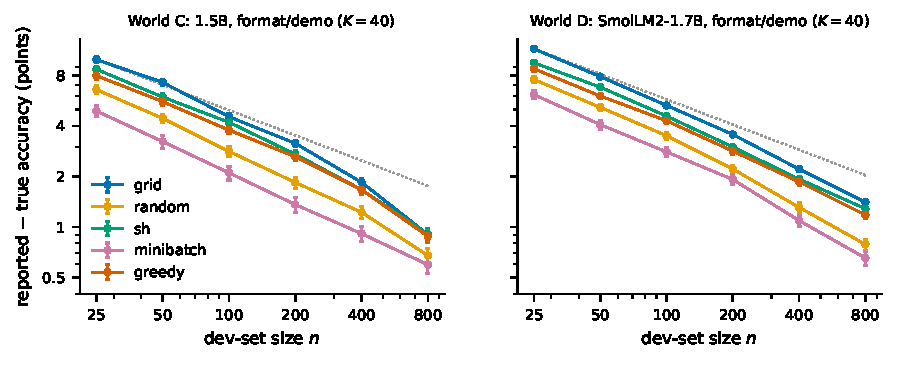
\includegraphics[width=.8\textwidth]{figs/gap_vs_n_extra.pdf}\caption{As \cref{fig:gap} for worlds C and D.}\end{figure}
\begin{table}[H]\caption{Reported $-$ true accuracy (points) by optimizer, worlds C and D.}\label{tab:gap_extra}\centering\scriptsize\setlength{\tabcolsep}{3pt}\begin{tabular}{lrrrr}\toprule
 & $n{=}50$ & 100 & 200 & 400 \\\midrule
\multicolumn{5}{l}{\emph{C: Qwen2.5-1.5B, format/demo grid ($K{=}40$)}} \\
Exhaustive & 7.3$\pm$0.3 & 4.5$\pm$0.2 & 3.1$\pm$0.1 & 1.8$\pm$0.1 \\
Random-8 & 4.4$\pm$0.3 & 2.8$\pm$0.2 & 1.8$\pm$0.1 & 1.2$\pm$0.1 \\
Succ. halving & 5.9$\pm$0.3 & 4.2$\pm$0.2 & 2.7$\pm$0.1 & 1.7$\pm$0.1 \\
Minibatch (MIPRO-like) & 3.2$\pm$0.3 & 2.1$\pm$0.2 & 1.4$\pm$0.1 & 0.9$\pm$0.1 \\
Greedy coord. & 5.6$\pm$0.3 & 3.8$\pm$0.2 & 2.6$\pm$0.1 & 1.7$\pm$0.1 \\
\multicolumn{5}{l}{\emph{D: SmolLM2-1.7B, format/demo grid ($K{=}40$)}} \\
Exhaustive & 7.9$\pm$0.2 & 5.3$\pm$0.1 & 3.6$\pm$0.1 & 2.2$\pm$0.1 \\
Random-8 & 5.2$\pm$0.2 & 3.5$\pm$0.2 & 2.2$\pm$0.1 & 1.3$\pm$0.1 \\
Succ. halving & 6.8$\pm$0.2 & 4.6$\pm$0.2 & 3.0$\pm$0.1 & 1.9$\pm$0.1 \\
Minibatch (MIPRO-like) & 4.1$\pm$0.2 & 2.8$\pm$0.2 & 1.9$\pm$0.1 & 1.1$\pm$0.1 \\
Greedy coord. & 6.0$\pm$0.2 & 4.3$\pm$0.2 & 2.8$\pm$0.1 & 1.9$\pm$0.1 \\
\bottomrule
\end{tabular}
\end{table}
\begin{table}[H]\caption{Reporting protocols, exhaustive search, $n{=}100$, worlds C and D (as \cref{tab:proto}).}\label{tab:proto_extra}\centering\scriptsize\setlength{\tabcolsep}{4pt}\begin{tabular}{lrrrr}\toprule
Protocol & bias & RMSE & coverage & width \\\midrule
\multicolumn{5}{l}{\emph{C: Qwen2.5-1.5B, format/demo grid ($K{=}40$)}} \\
Naive (dev score) & +4.5 & 6.2 & 0.85 & 18.3 \\
Holdout split (50/50) & +0.0 & 6.5 & 0.96 & 24.4 \\
5-fold cross-fit & -0.2 & 5.3 & -- & -- \\
Replay bootstrap (opt.) & +1.1 & 4.6 & -- & -- \\
Replay bootstrap (.632) & +1.4 & 4.6 & -- & -- \\
Empirical Bayes & +2.1 & 5.1 & 0.92 & 17.4 \\
Max-t simultaneous & +4.5 & 6.2 & 0.99 & 27.8 \\
Conditional (winner) & -7.1 & 16.9 & 0.77 & 25.1 \\
Ladder ($n^{-1/2}$) & +0.7 & 4.9 & -- & -- \\
\multicolumn{5}{l}{\emph{D: SmolLM2-1.7B, format/demo grid ($K{=}40$)}} \\
Naive (dev score) & +5.3 & 6.3 & 0.78 & 16.9 \\
Holdout split (50/50) & +0.2 & 5.7 & 0.95 & 21.6 \\
5-fold cross-fit & -0.1 & 4.9 & -- & -- \\
Replay bootstrap (opt.) & +1.4 & 3.9 & -- & -- \\
Replay bootstrap (.632) & +1.8 & 3.9 & -- & -- \\
Empirical Bayes & +0.8 & 3.7 & 0.97 & 16.2 \\
Max-t simultaneous & +5.3 & 6.3 & 0.99 & 26.0 \\
Conditional (winner) & -6.5 & 13.4 & 0.80 & 23.5 \\
Ladder ($n^{-1/2}$) & +1.4 & 4.2 & -- & -- \\
\bottomrule
\end{tabular}
\end{table}
\begin{table}[H]\caption{Claims, worlds C and D (as \cref{tab:concl}).}\label{tab:concl_extra}\centering\scriptsize\setlength{\tabcolsep}{2.5pt}\begin{tabular}{rrrrrrr}\toprule
$n$ & false claim & (holdout) & lift & holdout lift & A$-$B & (holdout) \\\midrule
\multicolumn{7}{l}{\emph{C: Qwen2.5-1.5B, format/demo grid ($K{=}40$)}} \\
50 & 0.25 & 0.03 & 7.0 / 0.1 & -0.4 & 3.6 / 0.2 & 0.0 \\
100 & 0.19 & 0.03 & 5.1 / 0.4 & 0.1 & 2.7 / 0.3 & 0.1 \\
200 & 0.14 & 0.02 & 3.8 / 0.7 & 0.4 & 2.0 / 0.4 & 0.2 \\
400 & 0.11 & 0.01 & 2.9 / 1.1 & 0.7 & 1.6 / 0.7 & 0.5 \\
\multicolumn{7}{l}{\emph{D: SmolLM2-1.7B, format/demo grid ($K{=}40$)}} \\
50 & 0.22 & 0.04 & 7.8 / -0.0 & -0.2 & 3.9 / 0.1 & -0.0 \\
100 & 0.18 & 0.03 & 5.6 / 0.3 & -0.0 & 2.8 / 0.3 & 0.3 \\
200 & 0.15 & 0.03 & 4.1 / 0.7 & 0.3 & 2.0 / 0.3 & 0.1 \\
400 & 0.11 & 0.02 & 3.1 / 1.0 & 0.7 & 1.6 / 0.4 & 0.3 \\
\bottomrule
\end{tabular}
\end{table}
\begin{table}[H]\caption{Sample splitting, worlds C and D (as \cref{tab:split}).}\label{tab:split_extra}\centering\scriptsize\setlength{\tabcolsep}{3pt}\begin{tabular}{lrrrrr}\toprule
Protocol & cost & bias & RMSE & cover. & width \\\midrule
\multicolumn{6}{l}{\emph{C: Qwen2.5-1.5B, format/demo grid ($K{=}40$)}} \\
no split (naive) & 0.0 & +4.5 & 6.2 & 0.85 & 18.3 \\
select on 30\% / report on 70\% & 0.80 & -0.1 & 5.5 & 0.95 & 20.8 \\
select on 50\% / report on 50\% & 0.38 & +0.0 & 6.5 & 0.96 & 24.4 \\
select on 70\% / report on 30\% & 0.18 & -0.2 & 8.4 & 0.95 & 30.8 \\
\multicolumn{6}{l}{\emph{D: SmolLM2-1.7B, format/demo grid ($K{=}40$)}} \\
no split (naive) & 0.0 & +5.3 & 6.3 & 0.78 & 16.9 \\
select on 30\% / report on 70\% & 0.62 & +0.1 & 4.7 & 0.94 & 18.3 \\
select on 50\% / report on 50\% & 0.38 & +0.2 & 5.7 & 0.95 & 21.6 \\
select on 70\% / report on 30\% & 0.15 & +0.2 & 7.6 & 0.94 & 27.4 \\
\bottomrule
\end{tabular}
\end{table}
\begin{table}[H]\caption{Uncertainty from the finite pool, worlds C and D (as \cref{tab:poolboot}).}\centering\scriptsize\setlength{\tabcolsep}{4pt}\begin{tabular}{lrrr}\toprule
world, $n$ & main design & pool-bootstrap mean & 95\% range \\\midrule
C, $n{=}50$ & 7.3 & 6.7 & 6.0--7.4 \\
C, $n{=}100$ & 4.5 & 4.4 & 3.8--5.0 \\
C, $n{=}400$ & 1.8 & 1.7 & 0.9--2.2 \\
D, $n{=}50$ & 7.9 & 7.4 & 6.6--8.1 \\
D, $n{=}100$ & 5.3 & 4.8 & 4.1--5.5 \\
D, $n{=}400$ & 2.2 & 1.7 & 1.0--2.3 \\
\bottomrule
\end{tabular}
\end{table}

\section{Compute, reproducibility and disclosures}
\label{app:repro}
\textbf{Compute actually used.} The environment provided a 4-core CPU quota (no GPU, no API). LLM scoring (fp32, 3--4 threads, sharing the quota with simulations, wall-clock from the run logs): world A (1.5B, $40\times750$ question-config pairs) $\approx$12 h; world B (0.5B) $\approx$3 h; world C (1.5B, format grid) $\approx$11 h; world D (SmolLM2-1.7B, $40\times450$) $\approx$8 h; i.e.\ about 34 h in total ($\approx$1.0--1.2 s per question-configuration pair for the 1.5B models). Simulation: about 1--1.3 h of one core per (world, 2000-episode gap experiment) plus minutes for the other experiments; synthetic sweeps $<$ 2 min. \textbf{Seeds}: pool seed 12345; demonstration-set seeds 777 (A) and 4242 (B--D); all simulations seed from an md5 hash of the setting (\texttt{exp\_main.py::seed\_of}); synthetic worlds use seeds 1, 2.
\textbf{Artifact map.} Table/figure $\to$ script: \cref{tab:worlds}, \cref{tab:gap}, \cref{tab:concl}, \cref{tab:proto}, \cref{tab:split}, \cref{tab:allopt,tab:norepl,tab:optsens} $\to$ \texttt{code/make\_tables.py} (inputs: \texttt{results/sim/*.parquet} from \texttt{code/exp\_main.py}); \cref{fig:gap,fig:effort,fig:theory,fig:concl,fig:ksweep,fig:protocols} $\to$ \texttt{code/make\_figs.py} (\cref{fig:theory}a,b from \texttt{code/exp\_synth.py}); Conditional-inference sanity check $\to$ \texttt{code/check\_cond.py}. See \texttt{README.md} for commands and expected run times.
\textbf{Negative and abandoned results.} (i) A llama.cpp CPU backend ran at $\approx$2 tokens/s here and was abandoned for torch fp32. (ii) World A turned out to be nearly flat (prompt differences of $\le$3 points, reliability $\approx 0$), which led us to add worlds B and A$\cup$B (real spread) and later C and D. (iii) The first SmolLM2 run was OOM-killed on 8-shot prompts (no grouped-query attention makes the expanded prefix cache large); we capped the cache size and resumed; world D uses 450 questions because that run was slower than planned (for $n$ near $N{=}450$ the i.i.d.\ pool design is less meaningful, so we report $n\le400$ for D). (iv) The first version of our empirical-Bayes interval (posterior sd) under-covered (0.45--0.72) and was replaced by the recentred interval of the main text; the first conditional-inference implementation mishandled exact ties (coverage 0.57--0.70) and was fixed by jittering (it still under-covers on discrete data); max-$t$ and EB for adaptive optimizers are heuristic; a trimmed-EB variant (restricting to near-winner configurations) helped only at large $n$ in A$\cup$B and was dropped. (v) We did not run DSPy/MIPRO themselves.
\textbf{Use of LLM assistance.} The research agent (an AI model) designed, ran and wrote up all of this work autonomously. \textbf{Content restrictions.} Literature was searched with scholarly-search tools only for classical statistics/ML references (winner's curse, cross-validation, post-selection inference, adaptive data analysis, prompt optimization); a search for ``optimizer's curse'' listed two 2025--2026 decision-analysis papers (policy evaluation), which were not opened. We did not intentionally search for, open or use the specific prior study the task excludes, and did not recognise any search result as such.
\textbf{Reproducibility checklist (ICML does not mandate one; provided for completeness).} Claims match results: yes (all numbers are produced by the listed scripts). Limitations: \cref{sec:discussion}. Theory assumptions/proofs: \cref{sec:setting}. Datasets, code, seeds, compute: this section and README. Error bars: 95\% CIs in tables/figures; coverage s.e.\ in captions. Statistical significance: Monte-Carlo s.e.; no hypothesis tests on the results themselves. Licenses: MMLU-Pro (MIT), Qwen2.5 (Apache-2.0 for 0.5B/1.5B). Human subjects: none.

\end{document}
